\chapterimage{RegulationsChapterImage.png} % Chapter heading image
\chapter{Regulations}
\section{Regulations Related to Wastewater Treatment}\index{Regulations Related to Wastewater Treatment}
The main objective of these regulations is to ensure appropriate quality of the treated wastewater.  

\subsection{Treated Wastewater - NPDES Permit}\index{Treated Wastewater - NPDES Permit}
The National Pollutant Discharge Elimination System (NPDES) permit program program addresses water pollution by regulating point sources that discharge pollutants to waters of the United States.

\begin{itemize}
\item The NPDES permit program was created in 1972 by the Clean Water Act (CWA)and is administered by the federal USEPA.
\item Applies to sources that discharge pollutants to waters of the United States.
\item Requires all facilities discharging “pollutants” into any body of water in the USA to obtain and comply with a \hl{NPDES permit}.
\item NPDES permit \hl{establishes} \textul{discharge limits}, \textul{monitoring} and \textul{reporting} \hl{requirements}\\
\item In California, the responsibility of implementing the federal NPDES program is delegated to the State of California through the State Water Resources Control Board (State Water Board or SWRCB) and finally to the nine Regional Water Quality Control Boards (Regional Water Boards or RWQCB), collectively known as Water Boards. 
\item The RWQCB issues the NPDES permit.
\end{itemize}

\subsection{Influent Wastewater - National Pretreatment Program}\index{Influent Wastewater - National Pretreatment Program}
Municipal wastewater treatment plants also known as Publicly Owned Treatment Works (POTWs) implement and enforce their Pretreatment or Industrial Discharge Control programs to meet Federal and State regulations requirements related to wastewater discharges from industrial sources.  The national pretreatment program is a component of the NPDES program and is also known as the Source Control Program\\

The Pretreatment/Source Control program is for controlling industrial (non-domestic) wastewater discharges with the following objectives:
\begin{enumerate}
\item Protect the treatment plant operations so that the industrial discharge does not contain pollutants or have certain characteristics (including pH, temperature) which could adversely effect the treatment process or impact public safety and the safety of the people working at the treatment plant.
\item Prevent the introduction of pollutants that could pass through untreated and into the receiving body of water.

\item Improve opportunities for reuse or recycling of wastewater and sewage sludge.

\end{enumerate}

In California:
\begin{enumerate}
\item Wastewater treatment plants are required to have a Pretreatment Program when their total design flows are greater than five million gallons per day (5 mgd). 
\item Facilities with smaller flows (5 mgd or less) may also be required to implement a Pretreatment Program if they receive industrial waste and pretreatment is warranted.
\item The Pretreatment Program for a wastewater treatment entity is reviewed and approved by the State and Regional Water Boards, and 
\item The Pretreatment Program's monitoring and reporting requirements are incorporated in the facility's NPDES permit.
\end{enumerate}

\section{Sewage Sludge/Biosolids Regulations}\index{Sewage Sludge/Biosolids Regulations}
Sewage sludge or biosolids is a byproduct of wastewater treatment.  The biosolids produced are disposed or used using methods including land application, landfill and incineration.  Federal Regulation 40CFR Part 503 also known as Rule 503 establishes the standards for the use or disposal of wastewater biosolids - as stipulated under the Clean Water Act.  The facility's NPDES permit incorporates the applicable federal, state and local requirements as they apply to its biosolids.
			\begin{itemize}
				\item Part 503 rule applies to any person who applies biosolids to the land or fires biosolids in a biosolids incinerator, and to the owner/operator of a surface disposal site, or to any person who is a preparer or generator of biosolids for use, incineration, or disposal.
				\item Part 503 standard includes:
					\begin{enumerate}
						\item General requirements which establishes the purpose and applicability of the rule, the compliance period, and exclusions from the rule.
						\item Limits on heavy metals content
						\item Solids management practices related to use and disposal of wastewater biosolids
						\item Operational standards related to biosolids management, and
						\item Requirements for the frequency of monitoring, record-keeping, and reporting
					\end{enumerate}
			\end{itemize}
Part 503 requirements are factored in when establishing the heavy metals concentration limits for the Pretreatment or Industrial Control Program as a significant portion of the heavy metals in the influent wastewater are removed as part of the wastewater solids.

\section{Air Quality Regulations}\index{Air Quality Regulations}
\begin{itemize}
\item Air emissions from wastewater collections and treatment systems are subject to federal, state and local air quality related rules and regulations established to protect human health and comfort, and the environment.  
\item Typically, a local agency such as the South Coast Air Quality Management District (SCAQMD) is designated to enact and enforce air quality rules and regulations, through its permitting process, applicable to all sources of air emissions including wastewater treatment plants.\\

\item Systems/processes subject to air quality regulations at air quality regulations include:

\begin{itemize}
\item Fugitive emissions:  Foul air containing compounds such as hydrogen sulfide and organics, which escape from process tanks, pipes and associated structures such as manholes and wetwells, is potentially harmful for the affected public and also cause odors.  
\item Digester gas combustion:  Digester gas a product of wastewater solids treatment contains methane and is either combusted in power generation equipment or burned in flares.
\item Odor control systems:  These commonly used systems are for controlling emissions of regulated pollutants such as ammonia and to prevent odors associated with compounds such as hydrogen sulfide.
\end{itemize}
 
\item Related to its air pollutants emissions, wastewater treatment plants are required to:
\begin{itemize}
\item Obtain air quality related operating permits for equipment and processes which emit air pollutants and for its systems treating foul air.
\item Implement air emission pollutants control measures
\item Comply with record keeping and reporting requirements
\item Comply with air quality rules to prevent public nuisance and protect public health and safety
\end{itemize}

\end{itemize}

\section{Regulations Related to Operations and Maintenance}\index{Regulations Related to Wastewater Treatment Operations and Maintenance}
\subsection{Operator Certification}\index{Operator Certification}
\begin{itemize}
\item The requirements of the Operator Certification program is established for each state.  These meet the Operator Certification Requirements of the regulations stemming from the 1996 Amendments to the Safe Drinking Water Act.
\item The goal is to ensure that operators of wastewater treatment facilities in the State meet the minimum level of competence; thereby, protecting public health and the environment.
\item In California, the Wastewater Operator Certification program (WWOCP) administers Wastewater Treatment Plant Certification examinations, certifications (grades I to V), and certification renewals. 
\item WWOCP classifies Wastewater Treatment Plants and stipulates that no person shall operate a wastewater treatment plant unless that person has been certified by the division as a wastewater treatment plant operator or operator-in-training at a grade appropriate for the class of plant being operated.
\item A certified operator or operator-in-training may be subject to administrative sanctions including reprimand or denial, suspension, probation, or revocation of the operator certification for performing, or allowing or causing another to perform acts which include:
\begin{itemize}
\item Operating or allowing the operation of a wastewater treatment plant by a person who is not certified at the grade necessary for the position
\item failing to use care or good judgment in the course of employment as an operator or failing to apply knowledge or ability in the performance of duties.
\item Negligence causing the violation of appropriate waste discharge requirements of the NPDES permit
\end{itemize}
\end{itemize}
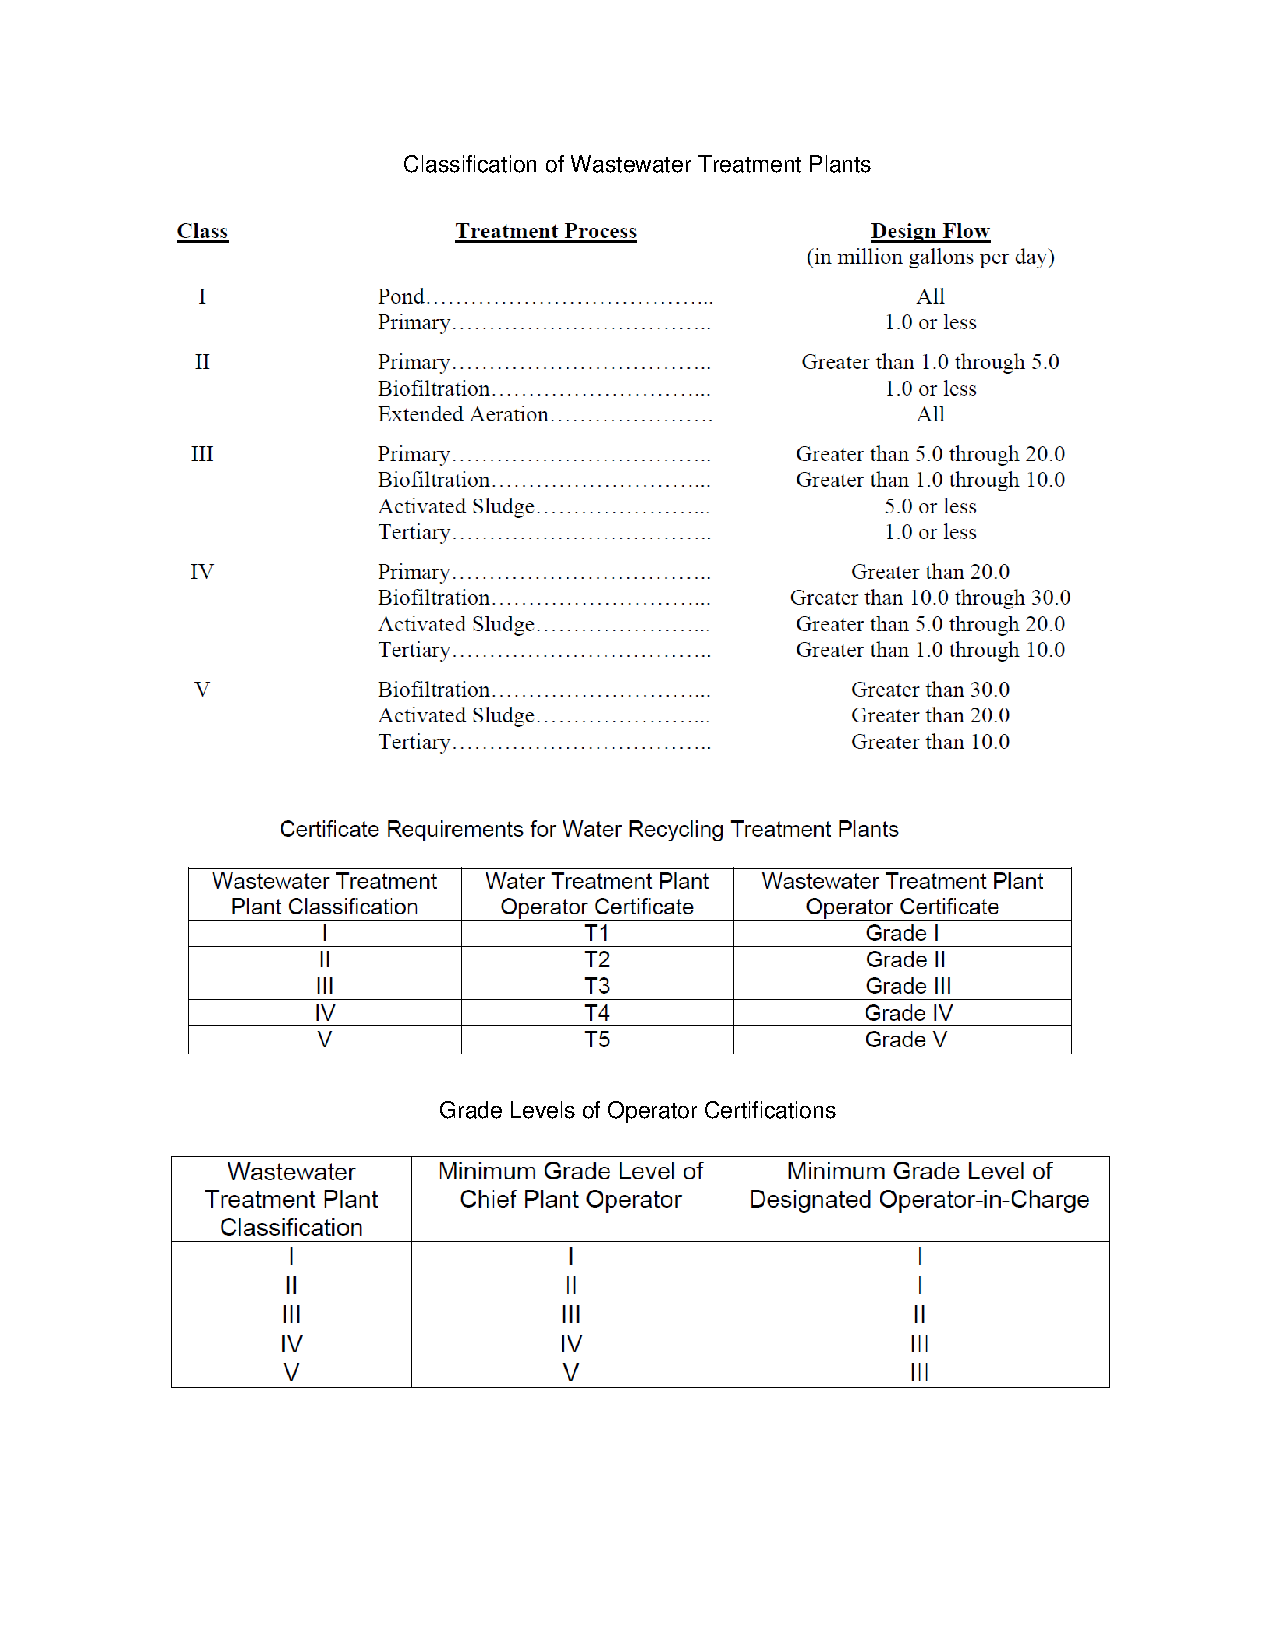
\includepdf[pages=-]{WastewaterPlantOperatorClassificationRequirements.pdf}
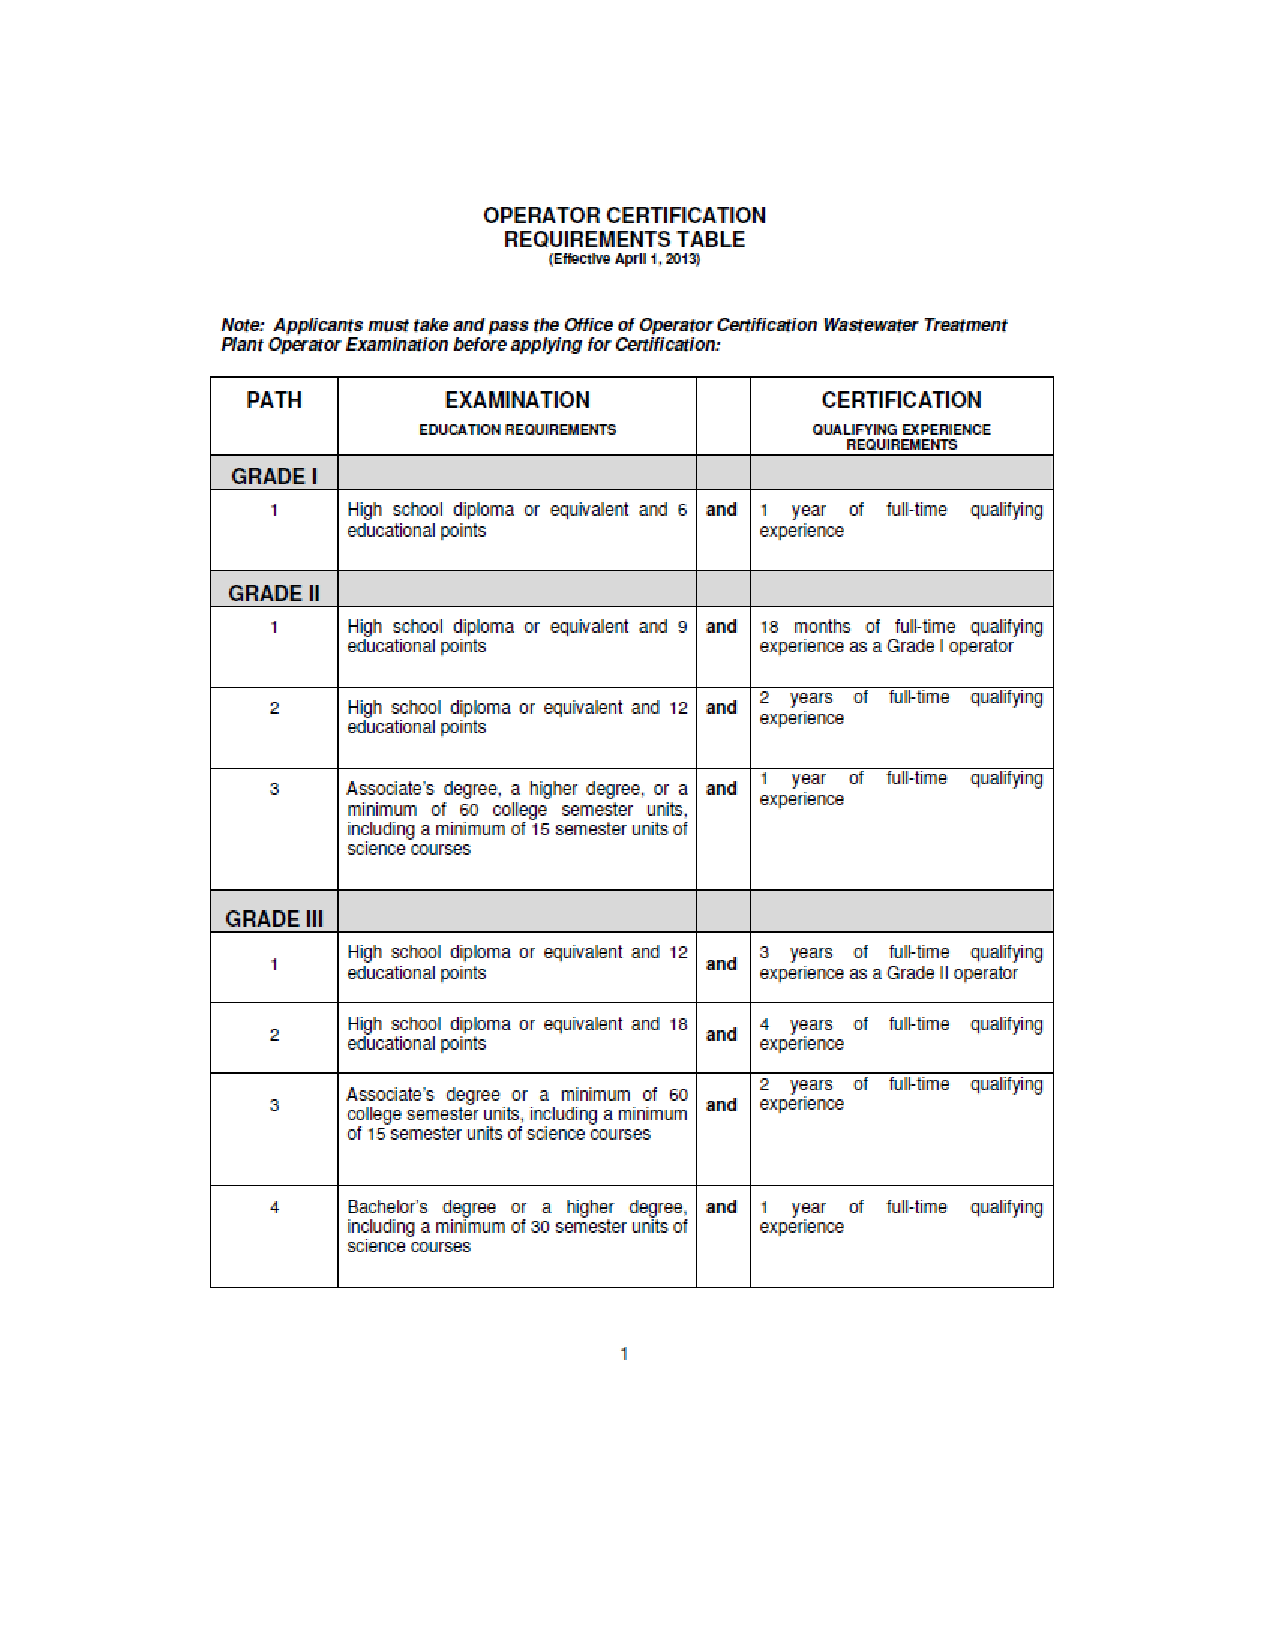
\includepdf[pages=-]{CertificationRequirement.pdf}

\subsection{Worker Safety}\index{Worker Safety}
\begin{itemize}
\item Wastewater treatment facility can be an extremely unsafe occupational field
\item It involves most of the major categories of workplace hazards:  biological, chemical, physical, safety and ergonomic,  accentuated with other factors such as shift work and diverse tasks.
\item Entities including The Occupational Safety and Health Administration(OSHA) National Electrical Code (NEC), National Fire Protection Association (NFPA), Underwriters Laboratory (UL) have recognized these hazards and implemented codes and standards to protect the affected persons and wastewater workers.
\end{itemize}
